% Options for packages loaded elsewhere
\PassOptionsToPackage{unicode}{hyperref}
\PassOptionsToPackage{hyphens}{url}
\PassOptionsToPackage{dvipsnames,svgnames,x11names}{xcolor}
%
\documentclass[
  letterpaper,
  DIV=11,
  numbers=noendperiod]{scrartcl}

\usepackage{amsmath,amssymb}
\usepackage{lmodern}
\usepackage{iftex}
\ifPDFTeX
  \usepackage[T1]{fontenc}
  \usepackage[utf8]{inputenc}
  \usepackage{textcomp} % provide euro and other symbols
\else % if luatex or xetex
  \usepackage{unicode-math}
  \defaultfontfeatures{Scale=MatchLowercase}
  \defaultfontfeatures[\rmfamily]{Ligatures=TeX,Scale=1}
\fi
% Use upquote if available, for straight quotes in verbatim environments
\IfFileExists{upquote.sty}{\usepackage{upquote}}{}
\IfFileExists{microtype.sty}{% use microtype if available
  \usepackage[]{microtype}
  \UseMicrotypeSet[protrusion]{basicmath} % disable protrusion for tt fonts
}{}
\makeatletter
\@ifundefined{KOMAClassName}{% if non-KOMA class
  \IfFileExists{parskip.sty}{%
    \usepackage{parskip}
  }{% else
    \setlength{\parindent}{0pt}
    \setlength{\parskip}{6pt plus 2pt minus 1pt}}
}{% if KOMA class
  \KOMAoptions{parskip=half}}
\makeatother
\usepackage{xcolor}
\usepackage[top=30mm,left=30mm]{geometry}
\setlength{\emergencystretch}{3em} % prevent overfull lines
\setcounter{secnumdepth}{-\maxdimen} % remove section numbering
% Make \paragraph and \subparagraph free-standing
\ifx\paragraph\undefined\else
  \let\oldparagraph\paragraph
  \renewcommand{\paragraph}[1]{\oldparagraph{#1}\mbox{}}
\fi
\ifx\subparagraph\undefined\else
  \let\oldsubparagraph\subparagraph
  \renewcommand{\subparagraph}[1]{\oldsubparagraph{#1}\mbox{}}
\fi


\providecommand{\tightlist}{%
  \setlength{\itemsep}{0pt}\setlength{\parskip}{0pt}}\usepackage{longtable,booktabs,array}
\usepackage{calc} % for calculating minipage widths
% Correct order of tables after \paragraph or \subparagraph
\usepackage{etoolbox}
\makeatletter
\patchcmd\longtable{\par}{\if@noskipsec\mbox{}\fi\par}{}{}
\makeatother
% Allow footnotes in longtable head/foot
\IfFileExists{footnotehyper.sty}{\usepackage{footnotehyper}}{\usepackage{footnote}}
\makesavenoteenv{longtable}
\usepackage{graphicx}
\makeatletter
\def\maxwidth{\ifdim\Gin@nat@width>\linewidth\linewidth\else\Gin@nat@width\fi}
\def\maxheight{\ifdim\Gin@nat@height>\textheight\textheight\else\Gin@nat@height\fi}
\makeatother
% Scale images if necessary, so that they will not overflow the page
% margins by default, and it is still possible to overwrite the defaults
% using explicit options in \includegraphics[width, height, ...]{}
\setkeys{Gin}{width=\maxwidth,height=\maxheight,keepaspectratio}
% Set default figure placement to htbp
\makeatletter
\def\fps@figure{htbp}
\makeatother

\KOMAoption{captions}{tableheading}
\makeatletter
\makeatother
\makeatletter
\makeatother
\makeatletter
\@ifpackageloaded{caption}{}{\usepackage{caption}}
\AtBeginDocument{%
\ifdefined\contentsname
  \renewcommand*\contentsname{Table of contents}
\else
  \newcommand\contentsname{Table of contents}
\fi
\ifdefined\listfigurename
  \renewcommand*\listfigurename{List of Figures}
\else
  \newcommand\listfigurename{List of Figures}
\fi
\ifdefined\listtablename
  \renewcommand*\listtablename{List of Tables}
\else
  \newcommand\listtablename{List of Tables}
\fi
\ifdefined\figurename
  \renewcommand*\figurename{Figure}
\else
  \newcommand\figurename{Figure}
\fi
\ifdefined\tablename
  \renewcommand*\tablename{Table}
\else
  \newcommand\tablename{Table}
\fi
}
\@ifpackageloaded{float}{}{\usepackage{float}}
\floatstyle{ruled}
\@ifundefined{c@chapter}{\newfloat{codelisting}{h}{lop}}{\newfloat{codelisting}{h}{lop}[chapter]}
\floatname{codelisting}{Listing}
\newcommand*\listoflistings{\listof{codelisting}{List of Listings}}
\makeatother
\makeatletter
\@ifpackageloaded{caption}{}{\usepackage{caption}}
\@ifpackageloaded{subcaption}{}{\usepackage{subcaption}}
\makeatother
\makeatletter
\@ifpackageloaded{tcolorbox}{}{\usepackage[many]{tcolorbox}}
\makeatother
\makeatletter
\@ifundefined{shadecolor}{\definecolor{shadecolor}{rgb}{.97, .97, .97}}
\makeatother
\makeatletter
\makeatother
\ifLuaTeX
  \usepackage{selnolig}  % disable illegal ligatures
\fi
\IfFileExists{bookmark.sty}{\usepackage{bookmark}}{\usepackage{hyperref}}
\IfFileExists{xurl.sty}{\usepackage{xurl}}{} % add URL line breaks if available
\urlstyle{same} % disable monospaced font for URLs
\hypersetup{
  colorlinks=true,
  linkcolor={blue},
  filecolor={Maroon},
  citecolor={Blue},
  urlcolor={Blue},
  pdfcreator={LaTeX via pandoc}}

\author{}
\date{}

\begin{document}
\ifdefined\Shaded\renewenvironment{Shaded}{\begin{tcolorbox}[breakable, enhanced, interior hidden, sharp corners, frame hidden, borderline west={3pt}{0pt}{shadecolor}, boxrule=0pt]}{\end{tcolorbox}}\fi

\hypertarget{vm303-01-studies-in-digital-media-culture}{%
\subsection{VM303-01 Studies in Digital Media \&
Culture}\label{vm303-01-studies-in-digital-media-culture}}

\begin{figure}

\begin{minipage}[t]{0.49\linewidth}

{\centering 

\raisebox{-\height}{

\href{https://instagram.com/dudewithsign/}{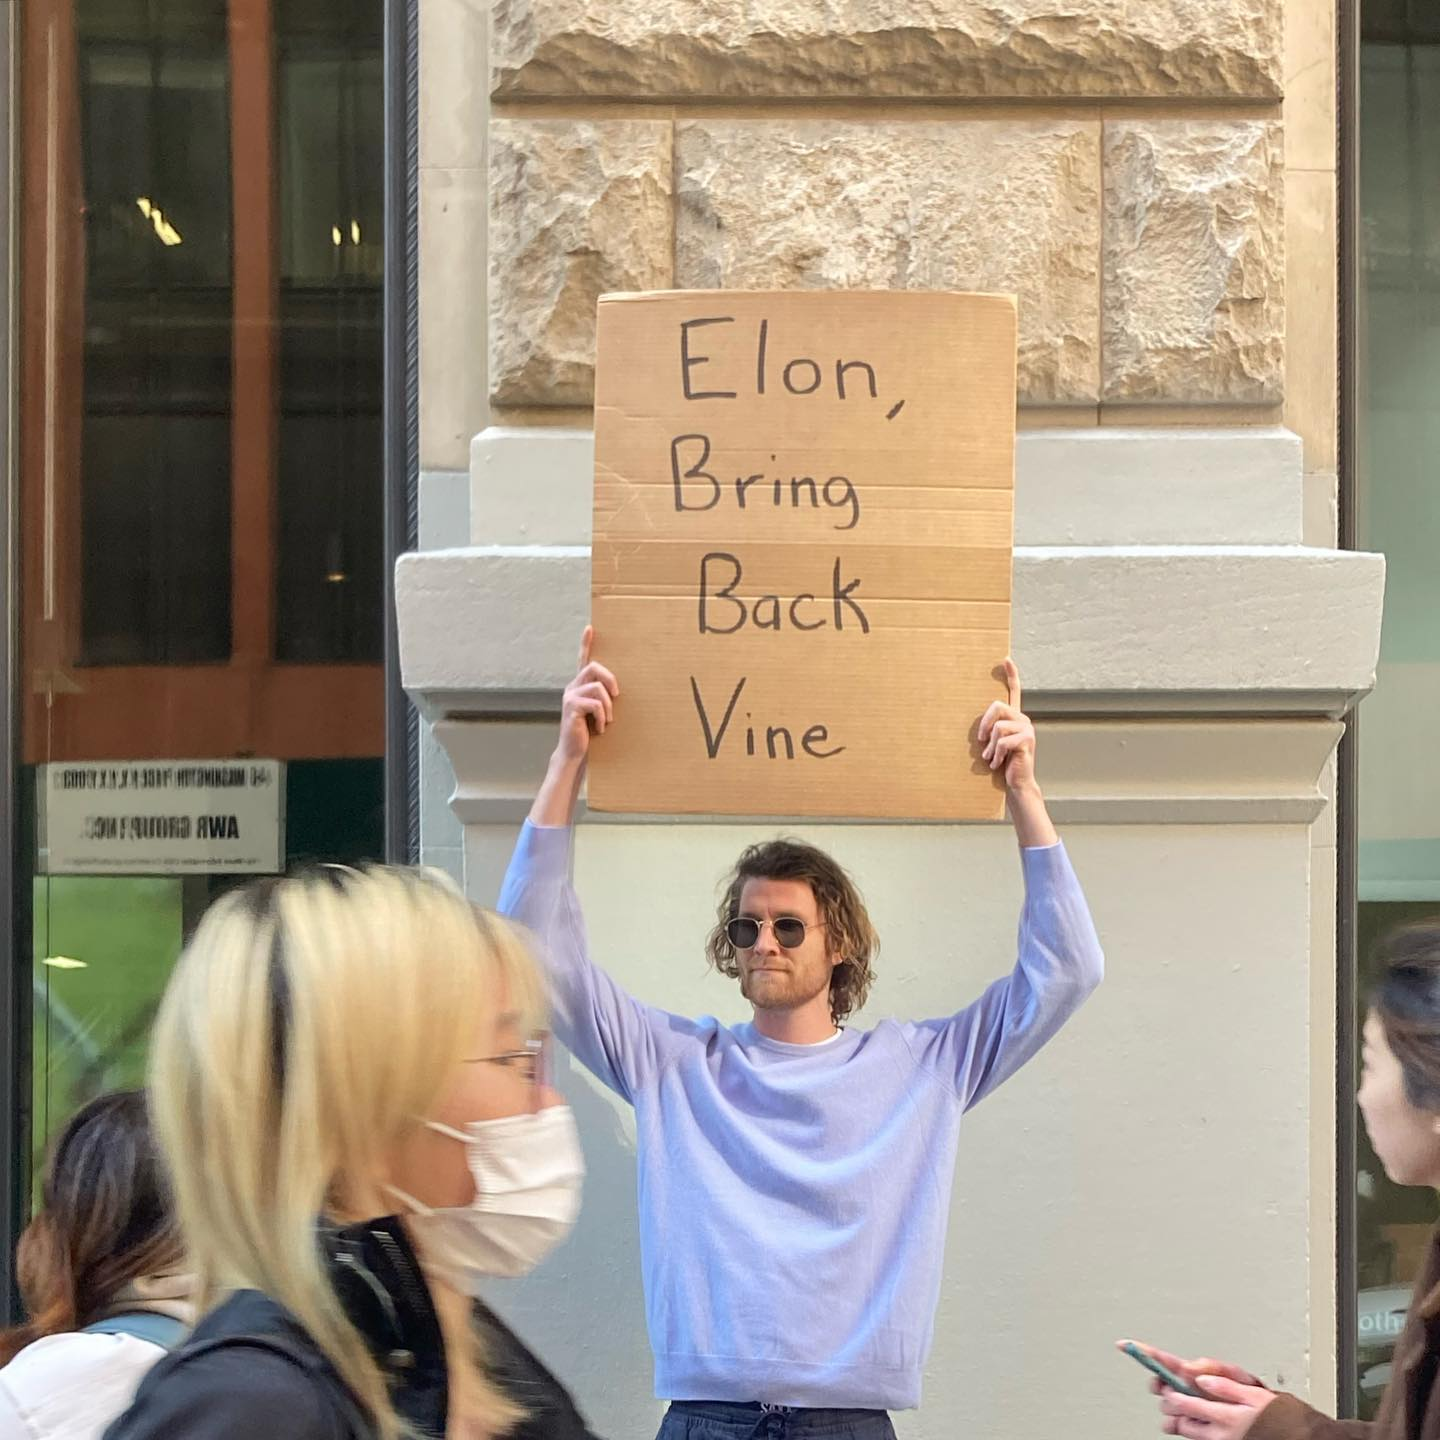
\includegraphics{img/dudewithsign.jpg}}

}

\caption{}

}

\end{minipage}%
%
\begin{minipage}[t]{0.02\linewidth}

{\centering 

~

}

\end{minipage}%
%
\begin{minipage}[t]{0.49\linewidth}

{\centering 

\href{https://emerson.edu/academics/academic-departments/visual-media-arts}{Department
of Visual \& Media Arts}\\
\href{https://emerson.edu/}{Emerson College}\\
Spring Semester 2023\\
Tues/Thur 17 January---4 May 2023 6:00-7:45 p.m.\\
Ansin 605\\
\href{http://mroberts.emerson.build/}{Dr.~Martin Roberts}\\
Office hrs: Thur 3:00-5:00 p.m.\\
Office: Ansin 915C\\
\href{https://www.youtube.com/playlist?list=PL3uFXkpHLYM7Qmw6Bw1tdTG0Th7xhrVHF}{YouTube
playlist} \textbar{}
\href{https://mroberts1.github.io/digital-culture-sp23/}{Syllabus}
(outside Canvas)\\

}

\end{minipage}%

\end{figure}

\begin{center}\rule{0.5\linewidth}{0.5pt}\end{center}

\href{https://www.youtube.com/playlist?list=PL3uFXkpHLYM7Qmw6Bw1tdTG0Th7xhrVHF}{YouTube
playlist} \textbar{}
\href{https://canvas.emerson.edu/courses/1932613/pages/mastodon-quickstart}{Mastodon
Quickstart} \textbar~

\textbf{Modules}:
\href{https://canvas.emerson.edu/courses/1932613/pages/w1-terminal-lucidity}{W1:
Terminal Lucidity} \textbar{}
\href{https://canvas.emerson.edu/courses/1932613/pages/w2-lurking}{W2:
Lurking} \textbar{}
\href{https://canvas.emerson.edu/courses/1932613/pages/w3-alternate-timelines}{W3:
Alternate Timelines} \textbar{}
\href{https://canvas.emerson.edu/courses/1932613/pages/w4-black-twitter}{W4:
Black Twitter} \textbar{}

\begin{center}\rule{0.5\linewidth}{0.5pt}\end{center}

\hypertarget{overview}{%
\subsubsection{Overview}\label{overview}}

This course considers the nature and contemporary forms of digital
culture. Broadly speaking, this can be defined as the diverse range of
symbolic practices through which communities affirm and maintain their
cultural identities using digital media devices and interfaces in a
globally networked society. While these practices are structured by
deeply unequal power relations, are contradictory, and often come into
conflict with one another, collectively they constitute what may be
considered a global digital culture.

A key component of the course is the automation of various forms of
creative production, from writing to the visual arts, by
natural-language processing computational systems (generally referred to
as ``artificial intelligence'' or ``AI''). The course addresses some of
the many issues raised by such systems, with a particular focus on
questions of aesthetics and the increasingly contested relationship
between artists and algorithms. While such systems now demonstrably pass
the Turing Test (i.e.~pass as human or their products as
human-produced), they also compel us to reconsider what we mean by
``art,'' or ``intelligence'' itself.

A major theme of the course is the changing status of the
\textbf{future} as a social imaginary. It has been suggested that while
we live today in the futures imagined by writers and filmmakers since
George Orwell's novel \emph{1984} (1949) and films like \emph{2001: A
Space Odyssey} (1968), \emph{Blade Runner} (1982, set in 2019 and later
2049), or \emph{Soylent Green} (1973, set in 2022), postmodern society
has become so absorbed in commemorating its own past that it has become
incapable of imagining its own future, dystopian or otherwise. As the
course shows, historical projections of the future (often referred to as
``retrofutures'') have paradoxically themselves become objects of
postmodernist nostalgia.

\begin{center}\rule{0.5\linewidth}{0.5pt}\end{center}

\hypertarget{chatgpt-summary}{%
\subsubsection{ChatGPT summary}\label{chatgpt-summary}}

This course that examines the diverse range of cultural practices that
use digital media and technology in a globally networked society. It
also focuses on the automation of creative production by artificial
intelligence systems and the implications that has on the meaning of art
and intelligence. The passage also notes that the course will examine
the changing perception of the future as a social imaginary, and how
society's focus on the past has affected our ability to imagine the
future.

\begin{center}\rule{0.5\linewidth}{0.5pt}\end{center}

\hypertarget{format}{%
\subsubsection{Format}\label{format}}

This is primarily a critical-thinking course, although it includes a
practical and production component. This means that it encourages you to
think reflexively and analytically about the digitally-mediated cultural
practices that the course considers, as well as to participate in them;
for example, you will be invited to experiment with image-synthesis and
text-generating software and analyze the results using key concepts and
theoretical frameworks.

\begin{center}\rule{0.5\linewidth}{0.5pt}\end{center}

\hypertarget{outcomes}{%
\subsubsection{Outcomes}\label{outcomes}}

By the end of the course, students will:

\begin{itemize}
\tightlist
\item
  have a acquired a deeper understanding of the social, cultural, and
  political dimensions of digital technologies and networked
  communication;
\item
  be able to apply critical thinking to contemporary developments in
  digital culture using relevant analytical concepts and both
  qualitative and quantitative methodologies such as cultural analytics;
\item
  understand basic principles of algorithmic image synthesis on a
  variety of platforms;
\item
  have reflected upon and discussed the larger significance of machine
  learning systems within global networked societies.
\end{itemize}

\begin{center}\rule{0.5\linewidth}{0.5pt}\end{center}

\hypertarget{texts}{%
\subsubsection{Texts}\label{texts}}

Selected chapters from the texts below will be made available as PDFs;
you are nevertheless encouraged to purchase at least several of texts
that are of interest and read more of them.

Note on formats: A number of texts listed in the bibliography are
available as e-books and/or audiobooks. You are encouraged to make use
not only of print media but also of these screen-based and audio
formats.

\href{https://mssv.net/}{Adrian Hon}, \emph{You've Been Played: How
Corporations, Governments, and Schools Use Games to Control Us All}. New
York: Basic Books, 2022.

\href{https://manovich.net/}{Lev Manovich} and Emanuele Arielli.
\href{http://manovich.net/index.php/projects/artificial-aesthetics-book}{\emph{Artificial
Aesthetics: A Critical Guide to AI, Media and Design}}. 2019-22.

\href{https://joannemcneil.com/}{Joanne McNeil}. \emph{Lurking: How A
Person Became A User}. New York: Farrar, Strauss, and Giroux, 2020.
ISBN: 978-1250785756.

\begin{center}\rule{0.5\linewidth}{0.5pt}\end{center}

\hypertarget{schedule-of-classes}{%
\subsubsection{Schedule of Classes}\label{schedule-of-classes}}

\begin{center}\rule{0.5\linewidth}{0.5pt}\end{center}

\emph{Week 1}

\textbf{I. Histories of the Future}

2023-01-17\_Tues

Alvy Ray Smith,
``\href{https://canvas.emerson.edu/courses/1932613/files/144544398?wrap=1}{A
Pixel Is \emph{Not} A Little Square, A Pixel Is \emph{Not} A Little
Square, A Pixel Is \emph{Not} A Little Square! (And a Voxel is
\emph{Not} A~ Little Cube)}''

\textbf{Terminal Lucidity}\\
Fisher,
``\,`\href{https://canvas.emerson.edu/courses/1932613/files/144544397?wrap=1}{The
Slow Cancellation of the Future}'\,''

Film: \emph{The Shining}\\
\emph{Everywhere at the End of Time} (The Caretaker)

2023-01-19\_Thur

\textbf{Internet Über Alles}\\
Hito Steyerl,
``\href{https://www.e-flux.com/journal/49/60004/too-much-world-is-the-internet-dead/}{Too
Much World: Is The Internet Dead?}'' (2013)
{[}\href{https://canvas.emerson.edu/courses/1932613/files/144544369?wrap=1}{pdf}{]}

Hito Steyerl,
``\href{https://www.e-flux.com/journal/10/61362/in-defense-of-the-poor-image/}{In
Defence of the Poor Image}'' (2009)
{[}\href{https://canvas.emerson.edu/courses/1932613/files/144727898?wrap=1}{pdf}{]}

\begin{center}\rule{0.5\linewidth}{0.5pt}\end{center}

\emph{Week 2}

2023-01-24\_Tues

\textbf{Lurking}\\
McNeil, \emph{Lurking}:
\href{https://canvas.emerson.edu/courses/1932613/files/144549946?wrap=1}{Introduction},
\href{https://canvas.emerson.edu/courses/1932613/files/144549950?wrap=1}{ch.~2}
(Anonymity)

2023-01-26\_Thur

McNeil, \emph{Lurking},
\href{https://canvas.emerson.edu/courses/1932613/files/144549949?wrap=1}{ch.~4}
(Sharing)

\begin{center}\rule{0.5\linewidth}{0.5pt}\end{center}

\emph{Week 3}

\textbf{Alternate Timelines}

2023-01-31\_Tues

Kaitlyn Tiffany,
``\href{https://canvas.emerson.edu/courses/1932613/files/145219877?wrap=1}{You
Probably Don't Remember The Internet}''

Choose and read \textbf{one} of these texts by
\href{http://www.instarbooks.com/remember-the-internet.html}{instar
books} (you will have to purchase either the print or ebook edition):

\begin{itemize}
\tightlist
\item
  Ana Valens,
  \href{http://www.instarbooks.com/books/tumblr-porn.html}{\emph{Tumblr
  Porn}}
\item
  Megan Milks,
  \href{http://www.instarbooks.com/books/tori-amos-bootleg-webring.html}{\emph{Tori
  Amos Bootleg Webring}}
\end{itemize}

2023-02-02\_Thur

\begin{itemize}
\tightlist
\item
  Quinn Myers,
  \href{http://www.instarbooks.com/books/google-glass.html}{\emph{Google
  Glass}}
\end{itemize}

\begin{center}\rule{0.5\linewidth}{0.5pt}\end{center}

\emph{Week 4}

2023-02-07\_Tues

Jason Parham,
``\href{https://www.wired.com/story/gadget-lab-podcast-514/}{Why The
History of Black Twitter Needed to be Told}'' (\emph{WIRED}, 30 July
2021). Please listen to the podcast on this page first, then read the
sections linked below.

Jason Parham,
``\href{https://www.wired.com/story/black-twitter-oral-history-part-i-coming-together/}{A
People's History of Black Twitter}'' (\emph{WIRED}, 29 July 2021)

\href{https://canvas.emerson.edu/courses/1932613/files/145300027?wrap=1}{Part
I} -
\href{https://canvas.emerson.edu/courses/1932613/files/145300043?wrap=1}{Part
II} -
\href{https://canvas.emerson.edu/courses/1932613/files/145300055?wrap=1}{Part
III}~

2023-02-09\_Thur

\textbf{The Angel of History: Afrofuturism}\\
Mark Dery, ``Black to the Future: Interviews with Samuel R. Delaney,
Greg Tate, and Tricia Rose,'' in \emph{Flame Wars: The Discourse of
Cyberculture} (Durham: Duke University Press, 1994

Kodwo Eshun, ``Further Considerations on Afrofuturism'' (\emph{The New
Centennial Review}, vol.~3, no. 2 (Summer 2003): 287-302)

Film (excerpt shown in class): \emph{The Last Angel of History} (John
Akomfrah/Black Audio Film Collective, 1995)

Jason Farago,
``\href{https://www.bbc.com/culture/article/20160401-how-klees-angel-of-history-took-flight}{How
Klee's `Angel of History' Took Flight}'' (BBC Culture, 6 April 2016)

``\href{http://www.africandigitalart.com/2017/10/05/the-futurist-digital-collages-by-manzel-bowman/}{The
Futurist Digital Collages of Manzel Bowman}''
(\href{http://africandigitalart.com/}{African Digital Art} website)

Recommended:
\href{https://mubi.com/films/the-african-desperate}{\emph{The African
Desperate}} (Martine Syms, 2022). Currently streaming on MUBI and Apple
TV

\begin{center}\rule{0.5\linewidth}{0.5pt}\end{center}

\emph{Week 5}

\textbf{DEADLINE: Alternate Timelines paper}

\textbf{II. Digital Imageworlds}

2023-02-14\_Tues

\textbf{Point-and-Shoot: Lo-fi Photography and Retro-Aesthetics}\\
Huang, Kalley.
``\href{https://www.nytimes.com/2023/01/07/technology/digital-cameras-olympus-canon.html?fbclid=IwAR1X2DutHJgtJFKB6XdcFjbm3kFB9P-IXPT7HckeGErsOrk0jTVGxugXYzk\&referringSource=articleShare\&smid=nytcore-ios-share\&unlocked_article_code=AAAAAAAAAAAAAAAACEIPuonUktbfqIhkSVUbBCbJUNMnqBqCgvfeh7A9iX7iJSzQQj9Hwv4cGM2H_1bIfbd4ItA62TOdAt9dNbtlDNpD8thiBW0_AQ-5vsnD350fPyQ-rY_0Dm9qhMvBUL59-jTjPizkd7wmgezgtErDOzbvUaLc2CB2LF1isoIlIQ_xoQEAxqjPGuB009hsj7x2Vt0hG2B2NGTdtOLoCh5_JNyFchjZjwE8UOhdUjzQ9sWOv_NCKE4BTAKbEw4spDo0-9heO9kIPa7gLBZGeMv2gLoZD2cAP55OPFabG3prPPkN94E3_vHG}{The
Hottest Gen Z Gadget Is a 20-Year-Old Digital Camera}''

``\href{http://ivc.lib.rochester.edu/snapshot-aesthetics-and-the-strategic-imagination/}{Snapshot
Aesthetics and the Strategic Imagination}''

2023-02-16\_Thur

\textbf{Soft Images: From Photograph to Database}\\
Horning,
``\href{https://robhorning.substack.com/p/the-expanded-field}{The
Expanded Field}''

Hoelzl and Marie, ``Expanded Photography (The Desire for Endlessness)''
in \emph{Softimage})

``\href{https://openai.com/blog/dall-e-introducing-outpainting/}{DALL-E:
Introducting Outpainting}''

\begin{center}\rule{0.5\linewidth}{0.5pt}\end{center}

\emph{Week 6}

2023-02-21\_Tues NO CLASS (Mon schedule)

2023-02-23\_Thur

\textbf{Object Detection}\\
Watch: \emph{Dragonfly Eyes} (Xu Bing, 2017)

Hatis Noit, ``Aura'' (music video)

\begin{center}\rule{0.5\linewidth}{0.5pt}\end{center}

\emph{Week 7}

\textbf{DEADLINE: ChatGPT Project}

\textbf{III. Algorithmic Aesthetics}

2023-02-28\_Tues

\textbf{The Sorcerer's Apprentice: AI Art}\\
Manovich, ``Who is an Artist in AI Era?''
(\href{http://manovich.net/index.php/projects/artificial-aesthetics-book}{\emph{Artificial
Aesthetics}}, ch.~2)

\textbf{Workshop: Midjourney}\\
\href{https://www.midjourney.com/}{Midjourney}: AI image synthesis

Guy Parsons,
``\href{https://dallery.gallery/midjourney-guide-ai-art-explained/}{Everything
you wanted to know about Midjourney}'' (5 August 2022)\\
\href{https://midjourney.gitbook.io/docs/}{Midjourney documentation}

2023-03-02\_Thur

\textbf{Magic Spells} Roland Barthes, ``Rhetoric of the Image''

\textbf{Workshop:}
\href{https://canvas.emerson.edu/courses/1932613/files/144544393?wrap=1}{DALL-E
2 Prompt Book}, \href{https://lexica.art/}{Lexica},
\href{https://www.reddit.com/r/promptcraft/}{promptcraft}

\begin{center}\rule{0.5\linewidth}{0.5pt}\end{center}

\emph{Week 8}

2023-03-07\_Tues

Lev Manovich, ``AI and Myths of Creativity''
(\href{http://manovich.net/index.php/projects/artificial-aesthetics-book}{\emph{Artificial
Aesthetics}}, ch.~4)

\textbf{Workshop: DALL-E 2}\\
\href{https://openai.com/dall-e-2/}{DALL-E 2}\\
\href{https://dallery.gallery/}{dall-ery gall-ery}

2023-03-09\_Thur

\textbf{Workshop: Stable Diffusion}\\
\href{https://stablediffusionweb.com/}{Stable Diffusion}

\begin{center}\rule{0.5\linewidth}{0.5pt}\end{center}

2023-03-13-17 \textbf{Spring Break}

\begin{center}\rule{0.5\linewidth}{0.5pt}\end{center}

\emph{Week 9}

\textbf{DEADLINE: Generative Art Project}

\textbf{IV. Gamification}

2023-03-21\_Tues

\textbf{Gaming The System}\\
Hon, \emph{You've Been Played}: Introduction, chapter 1

2023-03-23\_Thur

\textbf{The Gamified Self}\\
Hon, \emph{You've Been Played}: chapter 2

\begin{center}\rule{0.5\linewidth}{0.5pt}\end{center}

\emph{Week 10}

2023-03-28\_Tues

\textbf{Gamified Relationships: Ghosting}\\
Narr and Luong, ``Bored ghosts in the dating app assemblage: How dating
app algorithms couple ghosting behaviors with a mood of boredom''

Watch: \emph{The Tinder Swindler} (Netflix)

2023-03-30\_Thur

\textbf{Non-Player Characters: Gamifying the Workplace}\\
Hon, \emph{You've Been Played}: chapter 3

\begin{center}\rule{0.5\linewidth}{0.5pt}\end{center}

\emph{Week 11}

2023-04-04\_Tues

\textbf{The Gamified Society}\\
Hon, \emph{You've Been Played}: chapter 6 (Intro, The Myth and Reality
of the Social Credit Score, ``It Can't Happen Here,'' Propaganda,
Wargames)

2023-04-06\_Thur

Hon, \emph{You've Been Played}: chapter 6 (Elections, Civic Engagement,
Education)

\begin{center}\rule{0.5\linewidth}{0.5pt}\end{center}

\emph{Week 12}

\textbf{DEADLINE: Open Topic Analysis Paper}

2023-04-11\_Tues

\textbf{This Is Not A Game: ARGs}

Hon, \emph{You've Been Played}: chapter 7

Watch: \emph{The Institute}

2023-04-13\_Thur

\textbf{Gameworlds}

Hon, \emph{You've Been Played}: chapter 8

Watch: \emph{Free Guy}

\begin{center}\rule{0.5\linewidth}{0.5pt}\end{center}

\emph{Week 13}

2023-04-18\_Tues

Hon, \emph{You've Been Played}: chapters 9-10

2023-04-20\_Thur (Official make-up day, if necessary)

\begin{center}\rule{0.5\linewidth}{0.5pt}\end{center}

\emph{Week 14}

\textbf{DEADLINE: Gamification Projects}

2023-04-25\_Tues

Gamification Project Presentations

2023-04-27\_Thur

Gamification Project Presentations

\begin{center}\rule{0.5\linewidth}{0.5pt}\end{center}

\emph{Week 15}

2023-05-02\_Tues

Gamification Project Presentations

2023-05-04\_Thur \textbf{Last day of classes}

Gamification Project Presentations

\begin{center}\rule{0.5\linewidth}{0.5pt}\end{center}

\hypertarget{assignments-evaluation}{%
\subsubsection{Assignments \& Evaluation}\label{assignments-evaluation}}

\textbf{1. Alternate Timelines (15\%)}

Individual. Using the Alternative Timelines reading assignments as a
model, write a short paper of 1,000 words in length (4 pages
double-spaced, excluding bibliography) outlining your personal alternate
timeline of the internet.

\textbf{2. Open Topic Analysis Paper (15\%)}

Individual. Short paper analysis (1,000 words, 4 pages double-spaced) on
any of the topics discussed in the course to date (Week 12)

\textbf{3. Discussion forums (20\%)}

Individual. One or more discussion posts per week on reading
assignments, submitted anytime during the week of the assignments in
question. A minimum of ten weekly posts is required.

\textbf{4. ChatGPT (15\%)}

Individual. Write a prompt for ChatGPT (or a similar language-based
model) that generates a 500-word essay on a subject of your choice. (You
will likely have to experiment with customizing the prompt in order to
generate a satisfactory result.). Then write (do not generate) a
500-word reflection on the output from the prompt.

Remember that this output is the result of pattern matching from very
large datasets, not intelligence in the human sense; therefore, avoid
vague speculations about whether ChatGPT can be considered as
intelligent, or even sentient. Instead, evaluate the output purely
\textbf{as if} it was written by a human subject. How satisfactory is it
as a response to the prompt? What are its strengths, or blind spots? Can
it pass for having been written by a human? If not, why not? Is it
useful from a conceptual or analytical standpoint? If so, how?

\textbf{5.Generative Art Gallery (15\%)}

Individual. Using one of the systems focused on in the course (DALL-E 2,
Midjourney, Stable Diffusion), submit one work that was generated using
one of these systems. Images may be still or moving (e.g.~animations,
GIF loops, etc.)

Multiples are acceptable, even encouraged. This work will be reviewed
collectively by the group and displayed as a gallery, initally on
Canvas, and later (with your permission) on the web.

\textbf{6. Gamification Project (20\%)}

Group project (2-3 students).

Drawing on your reading of Adrian Hon's book \emph{You've Been Played},
in consultation with your other group members, develop a gamification
strategy for a product, service, organization, or institution of your
choice. This may be a real, existing product, etc., or one that does not
(yet) exist.

Write a proposal of approximately 1,000-1,500 words in length (4-6
pages, double-spaced) and prepare a presentation outlining the project
that you have in mind: primary objectives, target audience, platforms
used, game mechanics (how will people play it?), outcomes (points,
rewards, badges, leaderboards, etc). Projects will be presented and
discussed with the class during the last four meetings.

\begin{center}\rule{0.5\linewidth}{0.5pt}\end{center}

\hypertarget{bibliography}{%
\paragraph{Bibliography}\label{bibliography}}

{[}A{]} = audiobook (\href{http://audible.com/}{Audible.com})

Barthes, Roland. ``Rhetoric of the Image,'' in \emph{Image Music Text}.
Essays selected and translated by Stephen Heath. London: FontanaPress,
1977: 32-51.

Dery, Mark. ``Black to the Future: Interviews with Samuel R. Delaney,
Greg Tate, and Tricia Rose,'' in \emph{Flame Wars: The Discourse of
Cyberculture} (Durham: Duke University Press, 1994

Eshun, Kodwo. ``Further Considerations on Afrofuturism'' (\emph{The New
Centennial Review}, vol.~3, no. 2 (Summer 2003): 287-302)

Fisher, Mark. ``\,`The Slow Cancellation of the Future,'\,'' in
\emph{Ghosts of My Life: Writings on Depression, Hauntology and Lost
Futures}. Winchester, UK: Zero Books, 2014.

Hoelzl, Ingrid, and Rémi Marie. ``Expanded Photography (The Desire for
Endlessness),'' in \emph{Softimage: Towards A New Theory of the Digital
Image}. Bristol, UK: Intellect Books, 2015.

{[}A{]} \href{https://mssv.net/}{Hon, Adrian}. \emph{You've Been Played:
How Corporations, Governments, and Schools Use Games to Control Us All}.
New York: Basic Books, 2022.

Huang, Kalley.
``\href{https://www.nytimes.com/2023/01/07/technology/digital-cameras-olympus-canon.html?fbclid=IwAR1X2DutHJgtJFKB6XdcFjbm3kFB9P-IXPT7HckeGErsOrk0jTVGxugXYzk\&referringSource=articleShare\&smid=nytcore-ios-share\&unlocked_article_code=AAAAAAAAAAAAAAAACEIPuonUktbfqIhkSVUbBCbJUNMnqBqCgvfeh7A9iX7iJSzQQj9Hwv4cGM2H_1bIfbd4ItA62TOdAt9dNbtlDNpD8thiBW0_AQ-5vsnD350fPyQ-rY_0Dm9qhMvBUL59-jTjPizkd7wmgezgtErDOzbvUaLc2CB2LF1isoIlIQ_xoQEAxqjPGuB009hsj7x2Vt0hG2B2NGTdtOLoCh5_JNyFchjZjwE8UOhdUjzQ9sWOv_NCKE4BTAKbEw4spDo0-9heO9kIPa7gLBZGeMv2gLoZD2cAP55OPFabG3prPPkN94E3_vHG}{The
Hottest Gen Z Gadget Is a 20-Year-Old Digital Camera}.'' \emph{New York
Times}, 7 January 2023.

\href{https://manovich.net/}{Manovich, Lev}, and Emanuele Arielli.
\href{http://manovich.net/index.php/projects/artificial-aesthetics-book}{\emph{Artificial
Aesthetics: A Critical Guide to AI, Media and Design}}. 2019-22.

\href{https://joannemcneil.com/}{McNeil, Joanne}. \emph{Lurking: How A
Person Became A User}. New York: Farrar, Strauss, and Giroux, 2020.
ISBN: 978-1250785756.

Mumford, Lewis. ``Authoritarian and Democratic Technics,''
\emph{Technology and Culture} 5, no. 1 (Winter 1964): 1--8.
https://doi.org/10.2307/3101118.

Narr, Greg, and Anh Luong, ``Bored ghosts in the dating app assemblage:
How dating app algorithms couple ghosting behaviors with a mood of
boredom.'' \emph{The Communication Review}, 5 October.
https://doi.org/10.1080/10714421.2022.2129949

``\href{http://ivc.lib.rochester.edu/snapshot-aesthetics-and-the-strategic-imagination/}{Snapshot
Aesthetics and the Strategic Imagination}''. \emph{InVisible Culture: An
Electronic Journal for Visual Culture}, 18 (10 April 2013).

{[}A{]} Tiffany, Kaitlyn. \emph{Everything I Need I Get From You: How
Fangirls Created the Internet as We Know It}. Farrar, Strauss \& Giroux,
2022. ISBN: 978-0374539184.

\begin{center}\rule{0.5\linewidth}{0.5pt}\end{center}

\hypertarget{policies}{%
\subsubsection{Policies}\label{policies}}

\begin{center}\rule{0.5\linewidth}{0.5pt}\end{center}

\hypertarget{academic-honesty}{%
\paragraph{Academic Honesty}\label{academic-honesty}}

It is the responsibility of all Emerson students to know and adhere to
the College's policy on plagiarism, which can be found
at~\href{https://emerson.edu/policies/plagiarism}{emerson.edu/policies/plagiarism}.
If you have any question concerning the Emerson plagiarism policy or
about documentation of sources in work you produce in this course, speak
to your instructor.

\begin{center}\rule{0.5\linewidth}{0.5pt}\end{center}

\hypertarget{diversity}{%
\paragraph{Diversity}\label{diversity}}

Every student in this class will be honored and respected as an
individual with distinct experiences, talents, and backgrounds. Issues
of diversity may be a part of class discussion, assigned material, and
projects. The instructor will make every effort to ensure that an
inclusive environment exists for all students. If you have any concerns
or suggestions for improving the classroom climate, please do not
hesitate to speak with the course instructor or to contact the Social
Justice Center at 617-824-8528 or by email
at~\href{mailto:sjc@emerson.edu}{\nolinkurl{sjc@emerson.edu}}.

\begin{center}\rule{0.5\linewidth}{0.5pt}\end{center}

\hypertarget{discrimination-harassment-or-sexual-violence}{%
\paragraph{Discrimination, Harassment, or Sexual
Violence}\label{discrimination-harassment-or-sexual-violence}}

If you have been impacted by discrimination, harassment, or sexual
violence, I am available to support you, and help direct you to
available resources on and off campus. Additionally, the Office of Equal
Opportunity (\href{mailto:oeo@emerson.edu}{\nolinkurl{oeo@emerson.edu}};
617-824-8999) is available to meet with you and discuss options to
address concerns and to provide you with support resources. Please note
that I because I am an Emerson employee, any information shared with me
related to discrimination, harassment, or sexual violence will also be
shared with the Office of Equal Opportunity. ~If you would like to speak
with someone confidentially, please contact the Healing \& Advocacy
Collective, the Emerson Wellness Center, or the Center for Spiritual
Life.

\begin{center}\rule{0.5\linewidth}{0.5pt}\end{center}

\hypertarget{accessibility}{%
\paragraph{Accessibility}\label{accessibility}}

Emerson is committed to providing equal access and support to all
students who qualify through the provision of reasonable accommodations,
so that each student may fully participate in the Emerson experience. If
you have a disability that may require accommodations, please contact
Student Accessibility Services (SAS)
at~\href{mailto:SAS@emerson.edu}{\nolinkurl{SAS@emerson.edu}}~or
617-824-8592 to make an appointment with an SAS staff member.

Students are encouraged to contact SAS early in the semester. Please be
aware that accommodations are not applied retroactively.

\begin{center}\rule{0.5\linewidth}{0.5pt}\end{center}

\hypertarget{writing-academic-resource-center}{%
\paragraph{Writing \& Academic Resource
Center}\label{writing-academic-resource-center}}

Students are encouraged to visit and utilize the staff and resources of
Emerson's Writing Center, particularly if they are struggling with
written assignments. The Writing Center is located at 216 Tremont Street
on the 5th floor (tel. 617-824-7874).

\begin{center}\rule{0.5\linewidth}{0.5pt}\end{center}

\hypertarget{in-class-recording}{%
\paragraph{In-Class Recording}\label{in-class-recording}}

Regardless of modality or whether this course is being recorded by the
College with the permission of the students for classroom purposes, this
class is considered a private environment and it is a setting in which
copyrighted materials, creative works and educational records may be
displayed. Audio or video recording, filming, photographing, viewing,
transmitting, producing or publishing the image or voice of another
person or that person's materials, creative works or educational records
without the person's knowledge and expressed consent is strictly
prohibited.~

\begin{center}\rule{0.5\linewidth}{0.5pt}\end{center}



\end{document}
